\documentclass[oneside,a4paper,12pt]{article}
\usepackage{graphicx}
\usepackage{amsmath}
\usepackage{listings}
\lstset{language=html}
\usepackage{array}
\usepackage{pdfpages}
%\usepackage{biblatex}
%\bibliographystyle{plain}
%\bibliography{rapport.bib}
\usepackage{hyperref}
\graphicspath{{~/templates/}, {../images/}}

\makeindex
\begin{document}
	\begin{titlepage}
		\includegraphics[width=4cm]{logopopo.png}
		\hspace*{\fill}
		\includegraphics[width=6cm]{logouniv.png}
		
		\begin{center}
			\vspace{1cm}
			\textbf{Projet Ingénieur}\\
			\vspace{1cm}
			\textbf{\LARGE Gestion automatique de Cookies}\\
			\vspace{1cm}
			\textbf{Maxence NEUS}\\
			\vspace{1cm}
			
			\vspace{2cm}
			\vspace{\fill}
			\small Tuteurs :
			
			Jeremie Dequidt - Naif Mehanna - Walter Rudametkin
			
			\normalsize
			\vspace{2em}
			\textbf{2022}\\
		\end{center}
	\end{titlepage}
	
	\tableofcontents
	\vfill
	\begin{abstract}
		Dans le cadre du Projet Ingénieur, mon sujet a été proposé par un doctorant de l'équie Spirals à Inria, Naif Mehanna, avec qui j'avais effectué mon stage de 4e année. 
		Ce projet vient d'un besoin qu'il a exprimé lors de ses recherches à Spirals d'automatisation de la gestion des cookies lors de crawling de pages web.
	\end{abstract}
	
	
	
\section{Cahier des charges}
\subsection{Contexte}
Dans le cadre de recherches incluant des problématiques de vie privée, il est parfois nécessaire de gérer les popup et bannières de gestion de ookies sur les sites à étudier, en effet il est intéressant d'observer l'impacte des choix de l'utilisateur sur le comportement du site.
Pour réaliser ces choix il existe une extension chrome, \href{https://github.com/cavi-au/Consent-O-Matic}{Consent-O-matic} qui propose 5 types de cookies qu'il est possible d'accepter ou refuser dans les paramètres de l'extension. Malheureusement, cette extension utilise des templates uniques à un CMP (Consent Management Provider) à la fois et n'est donc par défaut pas suffisement général dans sa détection et son traitement des popup pour des applications à l'étude d'un grand nombre de sites qui peuvent avoir des CMP divers et variés. En effet il faudrait réaliser à la main des templates pour chaque CMP qui n'est pas utilisé par défaut.
De plus le temps d'execution de l'algorithme ne convient pas à une utilisation automatisée pour des fins de recherche sur un nombre de sites conséquent.
\subsection{But du projet}
Suite à l'étude du besoin décrit ci-dessus, il est proposé de créer un outil permettant de gérer automatiquement tout type de popup de consentement au cookies sans avoir recours à une configuration manuelle.

Pour cela l'outil proposé devra :

\begin{itemize}
	\item Détecter la présence d'une bannière de consentement
	\item En utilisant les préférences préalablement remplies par l'utilisateur :
	\subitem Déterminer quels types de permissions peuvent être données
	\item Sur la bannière détecter les différents types de permissions demandées
	\item Intéragir avec la bannière pour appliquer les préférences déterminées
\end{itemize}

On ajoutera une contrainte sur la vitesse globale d'execution de l'outil dans le but de ne pas ralentir les tests automatiques pour lesquels il pourrait être utilisé.

Finalement, il serait idéal d'incorporer l'outil dans un plugin \href{https://github.com/puppeteer/puppeteer}{pupeteer} afin de faciliter et d'accélerer encore le processus de test automatique.
	
	\section{Planning prévisionnel}
	
	\section{Travail effectué}
	\subsection{Structuration de l'application}
	\label{structure}
	Suite à nos premières intéractions avec mes tuteurs, nous sommes parvenu à une première approche concernant le développement de l'application. Nous avons proposé les solutions suivantes concernant les différents points du cahier des charges :
	
	\begin{itemize}
		\item On détectera les bannières via une approche s'inspirant de l'extension "I Don't Care About Cookies"
		\item L'extension prendra en paramettre les préférences de l'utilisateur sous la forme d'une liste des catégories acceptées par l'utilisateur
		\item On utilisera une approche basée sur le Machine Learning et plus particulièrement du Natural Language Processing (NLP) pour faire resortir les catégories proposées sur la bannière
		\item On intéragira directement avec la page via les APIs chrome pour aller cliquer sur les éléments correspondants
	\end{itemize}

	Après un temps de recherche de mon côté pour me familiariser avec le sujet des bannières de cookies, la partie qui semble à première vue demander le plus de temps est la partie Machine Learning. En effet elle requierts une quantité importante de données pour que l'application qui en resulte soit efficace.
	
	L'intéraction avec la page est également un problème qui parrait nécessiter du Machine Learning pour être fonctionnel sans devoir implémenter manuellement une solution pour chaque bannière. Cependant on propose de se concentrer sur la partie NLP dans un premier temps.
	
	\subsection{Recherches préliminaires}
	
	Pour mieux apprehander le sujet, j'ai commencé par en apprendre plus sur la façon dont sont gérées les bannières de cookies. 
	Initiallement et suite aux discussions que l'on a eu avec mes tuteurs lors de la présentation du sujet, je me suis penché sur les recherches qui ont aboutis à l'extension "Consent-o-matic" \cite{consentomatic}.
	Dans le papier, les auteurs décrivent l'état déplorable des cookies sur internet et notamment la mauvaise représentaion de ce qui est effectivement fait lorsque l'utilisateur accepte ou refuse les cookies sur une page.
	
	Dans le cadre de leurs recherches, ils ont extrait 6 catégories de cookies qu'ils allaient pouvoir étudier :
	\begin{figure}[h]
		\centering
		\label{categories}
		\begin{itemize}
			\item Performance And Analytics
			\item Preference And Functionnality
			\item Selection And Reporting of Ads
			\item Selection And Reporting Of Content
			\item Storage And Access To Information
			\item Others
		\end{itemize}
		\caption{Catégories de cookies}
	\end{figure}
	
	Dans notre projet, on ne s'intéressera pas à ce que fait effectivement le site en fonction des cookies acceptés, nous utiliserons simplement les catégories ci-dessus pour organiser nos choix de cookies.
	
	Le papier comporte aussi une réflexion sur les Consent Management Providers (CMP). En effet les CMP offrent un service qui permet à un site d'utiliser une bannière de cookies customisable mais avec un template pré-conçu. De cette façon c'est le CMP qui s'occupe de s'assurer que la bannière est conforme aux lois concernant l'acceptation des cookies.
	On notera que ces lois sont extrêmement vagues surtout concernant les modalités d'acceptation des cookies, ce qui nous posera des problèmes pour la suite.
	
	En effet il existe un grand nombre de CMP (le papier \cite{consentomatic} se concentre sur 5 mais il en existe bien plus, notamment lorsque l'on prend en compte les sites hors Europe et Amérique du Nord) ce qui apporte une complexité considérable à notre projet, en effet chaque CMP a une structure différente et cela nous posera problèmes en \ref{Interaction}
	
	En second temps, je me suis également intéressé à l'extension "I Don't Care About Cookies" qui permet de faire simplement disparaître les bannières. J'en ai extrait plusieurs techniques de détection et de masquage des bannières que je développe en \ref{DetectionDeBannieres}
	
	\subsection{Collecte de données}
	\label{collecte}
	Comme dit précédament, notre approche Machine Learning nous impose de collecter une grande quantitié de données sur ce que l'on essai de classifier.
	Dans notre cas on se concentre sur la discrimination das différentes catégories de cookies, plus particulièrement, on veut un modèle qui puisse nous donner une catégorie parmis les 6 présentées en \ref{categories} à partir d'un libellé présent sur une page.
	
	Pour obtenir ce modèle, on doit tout d'abord collecter un échantillon représentatif des libellés que l'on peut rencontrer sur des pages web. On propose de dériver cet échantillon à partir d'une liste de sites qui constitue l'état de l'art en terme de recherches web \href{https://tranco-list.eu/}{tranco}.
	
	\subsubsection{Détection de bannières}
	\label{DetectionDeBannieres}
	Pour accélerer la collection des données, j'ai proposé de faire une étape intermédiaire qui consiste à parcourir la liste des pages web à l'aide d'un crawler et de détecter si une bannière de cookies est présente sur la page, de cette manière on élimine les pages qui ne nous intéressent pas pour l'étape suivante.
	
	Pour réaliser cette première passe, on a besoin d'une manière de détecter la présence d'une bannière sur la page. 
	Suite à mes recherches sur "I Don't Care About Cookies", j'ai extrait deux méthodes qui pourrait êtrent utilisées pour notre application.
	
	La première consiste à insérer du CSS sur la page, permettant à partir des sélecteurs repris manuellement sur les bannières, de masquer les bannières (par ajout d'une rêgle \lstinline|{display: none;}|) afin que l'utilisateur n'ai pas à intéragir avec.
	On peut donc récupérer les sélecteurs CSS qui sont utilisés dans l'extension pour les intégrer à notre crawler.
	
	La seconde consiste cette fois à intercepter les requêtes HTTP qui permettent aux sites de récupérer les code des bannières sur un site distant pour les intégrer à leur page.
	On a proposé la possibilité d'utiliser ces interception de requêtes afin de retrouver le code inscrit dans la requête sur la page. Cette approche n'as pas été retenue pour notre application à cause de sa complexité d'exécution.
	
	Finalement, la première méthode a été appliquée sur un crawler qui sauvegarde le contenu des bannières lorsqu'il en détecte une. On a fait tourner ce crawler sur le server Typhon de l'équipe Spirals afin d'assurer son fonctionnement continu pendant un temps suffisant pour la collecte de nos données.
	 
	\subsubsection{Collecte des libellés de catégories}
	Une fois les sites contenant des bannières sauvegardés, on dois passer à un processus manuel afin de classifer les libellés dans les différentes catégories.
	
	On passe donc à un crawler manuel, c'est à dire un script qui visite les sites un par un et qui laisse à l'utilisateur le temps de cliquer sur les éléments nécessaires pour obtenir les libellés que l'on cherche afin de les copier dans des fichiers correspondants aux catégories.
	
	Un léger problème est survenu lors de cette étape car certains sites ne permettent pas de sélectionner le contenu des libellés, pour pallier à cela, j'ai installé une extension qui permet de copier le contenu d'un élément sur une page, ce qui a accéléré légèrement le processus.
	
	Au final, cette étape a pris un temps considérable mais a été peu efficace. En effet j'ai observé que les sites détectés à l'étape précédente utilisaient bien souvant les mêmes CMP et donc si l'administrateur du site ne change pas les libellés par défaut (ce qui arrive beaucoup), alors un grand nombre des sites visités comportent en fait les mêmes titres pour les différentes catégories.
	Cela implique que malgré plus d'un millier de sites visités, la catégorie avec les plus de libellés différents n'en compte que 18.
	
	Nous pouvons donc déjà supposer que notre modèle final ne seras malheureusement pas suffisament performant pour notre application.
	 
	 
	\subsection{Modélisation}
	\label{training}
	
	Malgré la faible quantité de données, on a voulu tenter d'entraîner un modèle avec les données que l'on a afin de montrer ce qui serait possible.
	
	\subsubsection{Préprocessing}
	\label{preprocessing}
	Pour pouvoir entraîner un modèle, il nous faut encoder nos données (texte) de manière numérique. Pour cela l'état de l'art utilise l'algorythme BERT pour génerer des embedings. C'est à dire une représentation numérique du sens lié à un morceau de texte. Cet algorythme est utilisé par suffisament d'organismes qu'il existe des modèles préentraînés de celui-ci qui nous permettent de l'intégrer rapidement à nos projets. Dans notre cas on utilise un modèle de Microsoft (\href{https://github.com/microsoft/CodeBERT}{page git du modèle})
	
	Notre entraînement commence donc par le préprocessing de nos données en utilisant le modèle présentés. On peut donc enregistrer les représentations obtenues pour qu'elles servent d'entrée à notre modèle.
	
	\subsubsection{Entraînement du modèle}
	Une fois nos données encodées, notre problème se décrit comme un problème de classification classique. Mes tuteurs proposent ici d'expérimenter avec des configurations classiques de modèles qu'on entraîne rapidement.
	
	Le premier que l'on va étudier ici est le RandomForest qui représente une liste d'arbres de décision qui votent sur la classification à donner à l'entrée.
	
	En utilisant les bibliothèques d'sklearn sous python, on parvient à entraîner un tel modèle avec notre dataset.
	On obtient un modèle avec une précision de 0.57 ce qui implique que le modèle est correcte seulement 57\% du temps.
	
	\subsubsection{Augmentation du dataset}
	\label{trainingFinal}
	Nos résultats avec le dataset tel quel sont prévisiblement mauvais. Pour tenter d'obtenir un modèle plus robuste et plus précis, on propose d'augmenter le dataset.
	
	Pour cela on utilise un processus décrit par \cite{wei-zou-2019-eda} qui consiste à créer des variations sur le texte de départ en changeant des mots par des synonymes ou en les changeant de place dans la phrase.
	
	Le papier \cite{wei-zou-2019-eda} donne un script python qui permet d'appliquer leur algorythme à un dataset de texte quelconque. On utilise donc ce script pour augmenter le nombre de points de donnée utilisés par le modèle.
	
	On peut alors relancer un entraînement du modèle avec le nouveau dataset augmenté pour obtenir les métrics suivants :
	
	\begin{figure}[h]
		\centering
		\begin{tabular}{|c|c|c|}
			\hline
			dataset & nombre de points & précision\\
			\hline
			simple & 55 & 0.57\\
			\hline
			augmenté & 540 & 0.87\\
			\hline
		\end{tabular}
		\caption{Comparaison avec RandomTree}
	\end{figure}

	On peut ensuite entraîner des modèles différents avec notre dataset augmenté.
	\newpage
	\begin{figure}[h]
		\centering
		\begin{tabular}{|c|c|c|}
\hline
modèle & précision & f1 score\\ 
 \hline 
HistGradientBoostingClassifier & 0.9444 & 0.9592\\ 
 \hline 
GradientBoostingClassifier & 0.9166 & 0.9118\\ 
 \hline 
RandomForestClassifier & 0.9074 & 0.9071\\ 
 \hline 
ExtraTreesClassifier & 0.8981 & 0.9070\\ 
 \hline 
\end{tabular}
		\caption{Metrics pour 4 types de modèles}
	\end{figure}
	
	\subsection{Extension}
	Pour illustrer notre application, on propose ici une démonstration d'une extension relativement basique qui devrait à minima ressembler à ce qu'on a décrit en \ref{structure}.
	
	Pour réaliser la classification des labels, il nous faut intégrer un modèle entraîné en \ref{trainingFinal}. Or celui-ci est codé sous python, alors que l'extension tourne en JavaScript sur le navigateur. 
	Il nous faut donc réaliser une passerelle entre ces deux languages, par ailleur les problématiques de puissance de calcul disponible sur navigateur nous pousse à réaliser les calculs ailleur.
	
	La méthode prévilégiée en production à l'heure actuelle consiste à créer une API qui tourne sur des serveurs distants et qui est scalable (c'est à dire que l'on peut déployer sur un grand nombre de serveurs pour minimiser la latence entre le serveur et l'utilisateur). Ces APIs fonctionnent habituellement par requêtes HTTP/HTTPS à un serveur sur lequel tourne un preocessus qui exécute le modèle entraîné.
	Pour simplifier et étant donné que le serveur fonctionnera sur ma machine, on utilisera ici des Websocket. Ces Websocket se comportent exactement comme une socket classique en réseau, c'est à dire qu'elle créé un lien possible à d'autres Websocket accessibles via le réseau (dans notre cas localhost). Ces liens nous permettent de transmettre du texte directement depuis l'extension vers un processus sur ma machine qui fera la classification.
	
	L'extension se compose de la manière suivante :
	
	Un processus ("server") tourne sur la machine et expose un Websocket sur localhost, ce processus en python récupère sur la Websocket du texte au format : \lstinline|{"id": "id", "texte": "texte_a_classifier"}|
	
	Il passe ensuite le texte à classifier par le preprocessing décrit en \ref{preprocessing} puis au classifieur (pour la démo on utilise le modèle RandomForest entraîné en \ref{trainingFinal}). Il répond ensuite sur la Websocket avec un message de la forme \lstinline|{"id": "id", "category": "category"}| o\`u id est l'id passé en entrée et category est la sortie du modèle.
	
	L'extension détecte la présence d'une bannière de cookies avec la méthode décrite en \ref{DetectionDeBannieres} puis par un processus hardcodé pour le moment trouve les libellés des catégories.
	
	Elle envoie ensuite les libellés avec l'id de l'élément qui correspond sur la Websocket pour obtenir la classification du label.
	
	\label{Interaction}
	Lors de la réception d'un message sur la Websocket, l'extension vérifie si la catégorie reçue fait partie des catégories à accepter, et si c'est le cas navigue la page jusqu'au boutton qui correspond au label et clique simplement dessus pour accepter les cookies.
	
	\begin{figure}[h]
		\centering
		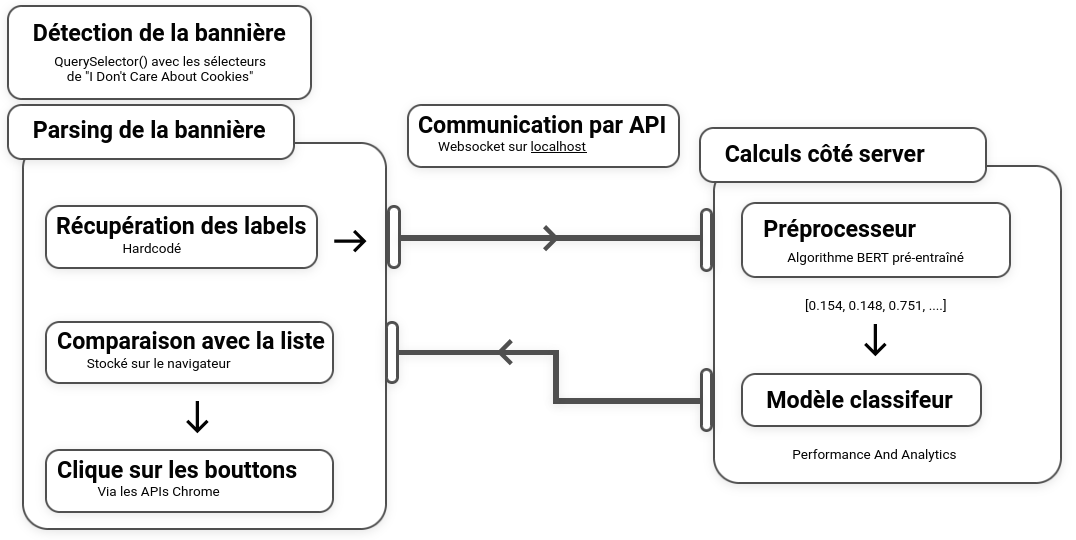
\includegraphics[width=\linewidth]{structure.png}
		\caption{Structure de l'extension}
	\end{figure}

	\section{Suites du projet}
	
	Plusieurs plans de l'application n'ont pas pu être traités dans les 8 semaines données au projet. Particulièrement, l'automatisation de la partie intéraction avec la bannière qui a été hardcodé dans la démo actuelle.
	
	\subsection{Intéractions avec la bannière}
	Nous pensons que la réalisation de cette partie va nécessiter du Machine Learning de la même façon que la partie de classification des labels. \`A la difference près que celle-ci utiliserai des features (points de données) de la structure HTML plutôt que l'approche NLP qu'on a eu jusqu'ici.
	
	Quelques pistes pour la conception de ce model :
	\begin{itemize}
		\item Par extraction de features par traitement du code HTML, potentiellement par un processus analogue à celui utilisé par mes camarades de stage dans le cadre de leurs recherches sur les pages de phishing \cite{phishing}
		\item Par une étude Machine Vision (c'est à dire par traitement d'images) sur une capture d'écran de la page web puis en utilisant l'outil d'inspection des éléments sur Chrome pour récuperer des éléments HTML avec lesquels intéragir.
	\end{itemize}
	
	\subsection{Classifieur}
	Pour ce qui est du classifieur, on voit deux méthodes à implémenter pour améliorer la précision du modèle.
	
	Tout d'abord comme on l'a noté dans la partie \ref{training} nous n'avons pas une quantité de données suffisantes pour obtenir une précision acceptable. La solution serait donc de collecter plus de données. Or comme on le verra ensuite, la méthode décrite en \ref{collecte} n'était pas aussi efficace qu'elle l'aurai pu. Par exemple en étudiant par avance la structure des bannières, on aurrait pu extraire simplement la partie qui liste les labels et obtenir une liste de labels que l'on aurait pu ensuite classifier directement plutôt que de naviguer sur chaque site manuellement.
	
	La seconde consiste à ajouter la description des cookies aux labels, ainsi on aurait plus de variations dans les couples $(label, description)$ que l'on avait avec simplement les labels.
	De plus, cette approche nous permet de prendre en compte des données plus complètes et donc améliorer notre compréhension de ce à quoi correspondent les catégories.
	
	\subsection{Intégration dans l'extension}
	
	L'extension dans son état actuel n'est qu'une démo permettant d'illustrer le concept. Une phase d'intégration de la solution reste à faire avant de pouvoir l'utiliser pour des recherches.
	Cette phase d'intégration comprends majoritairement la gestion de l'API de calcul.
	Actuellement, cette API tourne sur la machine de l'utilisateur ce qui, dans un cadre de déploiment chez les particuliers n'est pas viable. Une implémentation cloud serait aprioris la plus simple et rapide pour ce cas d'utilisation.
	
	Cepandent, dans le cadre de recherches où la puissance de calcul et la complexité d'installation sont moins un problème. On peut potentiellement réduire les temps de transmission des données et la latence en gardant le processus de calcul sur la machine afin de ne pas devoir passer par le réseau pour transmettre les packets à traiter.
	
	Des tests de latence et de performance sur l'aplication seront nécessaires pour déterminer laquelle de ces solutions est la plus adaptée.
		
	\section{Si c'était à refaire}
	
	Tout d'abord mes communications avec mes tuteurs ont fortement laissées à désirer pendant ce projet, c'est le point sur lequel j'ai le plus à travailler et l'avancée aurait pu être bien plus simple si elle avait été meilleure et si j'avais posé plus de questions à mes tuteurs nottament lors de la phase de collecte de données.
	
	En positif, je pense que la partie de recherches préliminaires m'as permis de bien comprendre le sujet et a été un investissement de temps utile.
	
	\`A mon avis notre choix de partir trés rapidement dans la collecte de donnée n'était pas le plus optimal, en effet peut-être qu'étudier la façon dont on pourrait intéragir avec la bannière avant de passer à la classification aurait pu nous permettre de collecter les données relatives à cette partie en même temps que celles nécessaires à la classification. Rendant ainsi le temps passé à la collecte de donnée plus rentable au final.
	
	Dans tout les cas, ce qui nous a fait perdre le plus de temps a été la collecte de données qui a malheureusement été infructueuse. En retrospective, j'aurai dû être plus proactif dans le questionnement du processus et ne pas tant m'attacher à obtenir une quantité suffisante de donnée avant de m'arrêter comme je l'ai fait.
	
	\newpage
	
	\begin{thebibliography}{9}
		\bibitem{consentomatic} Nouwens (2020): \emph{Dark Patterns after the GDPR: Scraping
Consent Pop-ups and Demonstrating their Influence}, Conference on Human Factors in Computing Systems
		
		\bibitem{wei-zou-2019-eda} Wei, Zou (2019): \emph{{EDA}: Easy Data Augmentation Techniques for Boosting Performance on Text Classification Tasks}, Conference on Empirical Methods in Natural Language Processing
		
		\bibitem{phishing} Aljofey, A., Jiang, Q., Rasool, A. et al. (2022): \emph{An effective detection approach for phishing websites using URL and HTML features}. Sci Rep 12, 8842 . https://doi.org/10.1038/s41598-022-10841-5 
	\end{thebibliography}

\end{document}